%% Document created 27 November 2021 automatically 
%% from /Users/massimosotgia/Desktop/uni_at_DIFI/Lab2/setup.py 

%% Copyright (C) Mattia Sotgia et al. 2022
%% Using class revtex4-2.cls

\documentclass[
    rmp,
    % preprint,
    % linenumbers,
    % tightlines,
    reprint, 
    superscriptaddress, 
    altaffilletter, 
    amsmath, 
    amssymb, 
    a4paper]{revtex4-2}

\usepackage[top=1.75cm,bottom=2.5cm,left=1.5cm,right=1.5cm]{geometry}

\usepackage[utf8]{inputenc}
\usepackage[T1]{fontenc}

\usepackage[italian]{babel}

%% revtex4-2 bug-fix
\def\andname{e}
%--------------------
\makeatletter
\let\it@comma@def\active@comma
\makeatother

\usepackage{txfonts}
\usepackage{graphicx}% Include figure files
\graphicspath{{../fig/}}

\usepackage{dcolumn}% Align table columns on decimal point
\usepackage{bm}% bold math
\usepackage[colorlinks, urlcolor=., bookmarks]{hyperref}% add hypertext capabilities
\renewcommand\UrlFont{\color{blue}}

\usepackage{physics}
\usepackage{siunitx}

\usepackage{fancyhdr}
\pagestyle{fancy}
\fancyhf{}
\def\twodigits#1{\ifnum#1<10 0\fi\the#1}

%-----------------------------------------------------------------------------------------------

\usepackage{background}
\SetBgColor{gray}
\SetBgAngle{90}
\SetBgScale{2}
\SetBgVshift{0.27\textwidth}

\usepackage[american resistors]{circuitikz}
\usepackage{listings}
\lstset{
  basicstyle=\fontsize{5}{6}\selectfont\ttfamily,
  % backgroundcolor=\color{white},   % choose the background color
  % basicstyle=\footnotesize,        % the size of the fonts that are used for the code
  breakatwhitespace=false,         % sets if automatic breaks should only happen at whitespace
  breaklines=true,                 % sets automatic line breaking
  captionpos=b,                    % sets the caption-position to bottom
  % commentstyle=\color{mygreen},    % comment style
  deletekeywords={...},            % if you want to delete keywords from the given language
  escapeinside={\%*}{*)},          % if you want to add LaTeX within your code
  % extendedchars=true,              % lets you use non-ASCII characters; for 8-bits encodings only, does not work with UTF-8
  % firstnumber=1000,                % start line enumeration with line 1000
  % frame=single,                    % adds a frame around the code
  % keepspaces=true,                 % keeps spaces in text, useful for keeping indentation of code (possibly needs columns=flexible). 
  % keywordstyle=\color{blue},       % keyword style
  % numbers=left,                    % where to put the line-numbers; possible values are (none, left, right)
  % numbersep=5pt,                   % how far the line-numbers are from the code
  numberstyle=\tiny\color{gray}, % the style that is used for the line-numbers
  % rulecolor=\color{black},         % if not set, the frame-color may be changed on line-breaks within not-black text (e.g. comments (green here))
  showspaces=false,                % show spaces everywhere adding particular underscores; it overrides 'showstringspaces'
  showstringspaces=false,          % underline spaces within strings only
  showtabs=false,                  % show tabs within strings adding particular underscores
  stepnumber=2,                    % the step between two line-numbers. If it's 1, each line will be numbered
  % stringstyle=\color{mymauve},     % string literal style
  tabsize=2,                       % sets default tabsize to 2 spaces
}
\usepackage{soul}


%% Define ref types
\newcommand{\reftab}[1]{Tabella {\ref{#1}}}%
\newcommand{\reffig}[1]{Figura {\ref{#1}}}%
\newcommand{\refeqn}[1]{({\ref{#1}})}%
\newcommand{\ChiSqr}{$\chi^2$\space}
\newcommand{\ChiNdf}{$\chi^2/\text{ndf}$}
\newcommand{\cernroot}{\texttt{root}}
\newcommand{\treSigma}{$3\sigma$}
\newcommand{\stdErr}[1]{$\varepsilon_{#1}$}
\newcommand{\mstdErr}[1]{\varepsilon_{#1}}
%% PAPER ONLY custom Macros

\newenvironment{methods}[1]{\section*{#1}
%\fontfamily{phv}
\fontsize{7.5}{9}\selectfont\label{sec:methods}\noindent}{\par\noindent}

%\usepackage{lcsec}

\sisetup{
    % separate-uncertainty=true,
    round-mode=uncertainty,
    % exponent-mode = scientific
}

\fancyfoot[C]{
    \the\year\twodigits\month\twodigits\day/4-\thepage
}
\fancyhead[C]{\fontfamily{phv}\fontsize{12}{12}\selectfont RELAZIONE DI LABORATORIO \textbf{
    N. 2 % ! <== CAMBIARE (Nessuna rel. -> 00)
    } (\the\year)
}

\newcommand{\LMopamp}{{\fontfamily{phv}\selectfont\small\bf LM741}}

\begin{document}

\title{- 
}
\thanks{Esperienza n. 4
}

\author{Francesco Polleri}
\email{s5025011@studenti.unige.it}
\author{Mattia Sotgia}
\email{s4942225@studenti.unige.it}

\collaboration{Gruppo A1}
\affiliation{Dipartimento di Fisica, Università degli Studi di Genova, I-16146 Genova, Italia}

\date{presa dati
    30 novembre, 1-2 dicembre 2021, consegnata in data 
    \today
}

\begin{abstract}
    
\end{abstract}
\maketitle
\thispagestyle{fancy}
% Rimuovere per consegna
\SetBgContents{
    laboratorio2: e4 (non per la consegna) \today % ! Note di versione
}

%%%% CORPO DEL TESTO
%%%% CORPO DEL TESTO

\section*{Introduzione}
Lo scopo principale di questa esperienza di laboratorio è fare una verifica sperimentale della dipendenza quadratica inversa dell'energia irradiata da una sorgente luminosa in funzione della distanza da essa.
Per fare le misure necessarie abbiamo bisogno di diversi dispositivi e in particolare, l'esperienza si basa sull'utilizzo degli amplificatori operazionali. 

Come sorgente luminosa usiamo una piccola lampadina ad incandescenza che possiamo posizionare a diverse distanze da un termometro al platino (PT100) che usiamo quindi come sensore e la cui caratteristica principale è la dipendenza lineare, a temperature intorno a quella ambiente, della resistenza in funzione della variazione di temperatura (la derivata è 0.4 \unit{\ohm/\kelvin}). 

Poiché vogliamo misurare delle variazioni di temperatura attraverso la variazione del valore di una resistenza, utilizziamo un ponte di Wheatstone in modo che le nostre misure siano il più precise possibili e per vedere ancora meglio gli effetti di queste variazioni sulla nostra uscita del segnale usiamo un amplificatore per strumentazione. 

\section*{Studio e caratterizzazione di un amplificatore operazionale}

Poiché l'amplificatore per strumentazione che utilizziamo per la nostra misura è costituito da tre amplificatori operazionali inseriti in un unico circuito, ci interessa studiare meglio il loro comportamento in modo da progettare il circuito nel modo migliore possibile.

\begin{figure}[b!]
    \begin{circuitikz}
        \draw (0,0)
        node[op amp, scale=0.5] (opamp) {}
        (opamp.-) to [short, -*] (-1, 0.25)
        to [R, l^=$R_{1}$, resistors/scale=0.8] node[left]{in}(-2.5, 0.25)
        (-1, 0.25) -- (-1, 1) to [R, l=$R_{2}$, resistors/scale=0.8](1, 1)
        to [short, -*] (1, 0)
        (opamp.out) -- (2,0) node[right]{out}(2, 0)
        (opamp.+) -- (-1, -0.25) -- (-1, -0.75) node[ground]{}
        ;
    \end{circuitikz}
    \caption{Schema circuitale amplificatore invertente}
    \label{fig:amp_inv}
\end{figure}

Iniziamo costruendo un semplice circuito (\reffig{fig:amp_inv}) con un amplificatore \LMopamp alimentato con $\pm V_{cc}=\pm 15V$ e progettato in modo che il guadagno ad anello chiuso sia $G_{\text{close}}=80$. Attraverso lo studio del circuito troviamo che il guadagno risulta essere $G=-\frac{R_{1}}{R_{2}}$. Per scegliere le resistenze da inserire nel circuito non ci basiamo però solo su questa condizione, bensì le prendiamo in modo che siano molto più grandi della resistenza interna del generatore che dovrebbe essere circa \SI{50}{\ohm}. Prendiamo quindi come valore nominale di $R_{1}$ \SI{1}{\kilo\ohm}, mentre per $R_2$ \SI{80}{\kilo\ohm}. Misuriamo le resistenze con il tester a nostra disposizione e troviamo che $R_{1}=\SI{0.988 +- 0.006}{\kilo\ohm}$ mentre $R_{2}=\SI{82.7 +- 0.5}{\kilo\ohm}$ 

Per effettuare la misura del guadagno raccogliamo 5 valori della tensione di uscita ($V_{out}$) con i rispettivi valori della tensione di entrata ($V_{in}$) a \SI{50}{\hertz} in modo da acquisire i dati in ua zona in cui il guadagno non dipende dalla frequenza poichè l'amplificatore si comporta come un passa basso  .Inoltre i valori di $V_{in}$ li abbiamo scelti in modo che, una volta amplificati, fossero comunque minori di $15V$, che è la tensione con cui alimentiamo l'amplificatore, perchè altrimenti il valore di $V_{out}$ sarebbe appunto uguale a $V_{cc}$ (questi valori sono riportati in \reftab{??}). Eseguendo in fit lineare usando come funzione \[V_{out}=G\cdot V_{in}+q\] e impostando come parametri $G$ e $q$ Otteniamo quindi che 
\begin{align*}
    G & =\num{78.6454 +- 8.1} \\
    q & =\SI{0.03}{\volt} \\ 
\end{align*}

Osserviamo quindi che il valore di $G$ è compatibile con il valore che volevamo ottenere, cioè $G=80$ e che la quota della retta è compatibile con zero e ciò rispecchia il fatto che se la tensione in entrata è nulla, anche quella in uscita deve esserlo.

Utilizzando sempre lo stesso circuito vogliamo creare un diagramma di Bode della funzione di trasferimento, in modo da osservare effettivamente il comportamento da passa-basso e da trovare la frequenza di taglio. Impostiamo quindi la $V_{in}$ a $100mV$ e raccogliamo i valori di $V_{in}$, $V_{out}$ e del periodo $T$ con i loro rispettivi fondo scala, facendo variare la frequenza da 100Hz fino 20KHz raccogliendo circa 3 punti per ogni decade (questi valori sono riportati in \reftab{??}). Realizziamo un fit sui dati usando come funzione  \begin{equation}\left|H[\nu]\right|=\frac{G}{\sqrt{1+\left(\frac{\nu}{\nu_0}\right)^2}} \label{eq:H}\end{equation} e scegliendo come parametri $G$ e $\nu_0$. 
Otteniamo quindi che
\begin{align*}
    G     &=\num{ 83.2458 +- 1.24581} \\
    \nu_0 &=\SI{8.71835 +- 0.2559}{\kilo\hertz} \\ 
\end{align*}

Ripetiamo lo stesso procedimento utilizzando però come $R_2$ una resistenza da \SI{8}{\kilo\ohm} in modo che il guadagno sia 10 volte più piccolo. Vogliamo quindi verificare che il prodotto $\nu_0 \cdot G $ è costante. Raccogliamo quindi i nuovi dati riportati in \reftab{??} e realizziamo un altro fit usando di nuovo l'equazione \refeqn{eq:H} e impostando gli stessi parametri e troviamo che
\begin{align*}
    G     &=\num{7.99818 +- 0.101188} \\
    \nu_0 &=\SI{85.4452 +- 2.31586}{\kilo\hertz} \\ 
\end{align*}
Osserviamo che effettivamente il guadagno si presenta essere circa 10 volte più grande del valore misurato in precedenza.

Nel primo caso il prodotto vale \num{68.3406 +- 2.04412e4}, mentre nell'altro caso vale \num{72.5766 +- 2.39117e4} e troviamo che quindi sono effettivamente compatibili.

\begin{figure}
    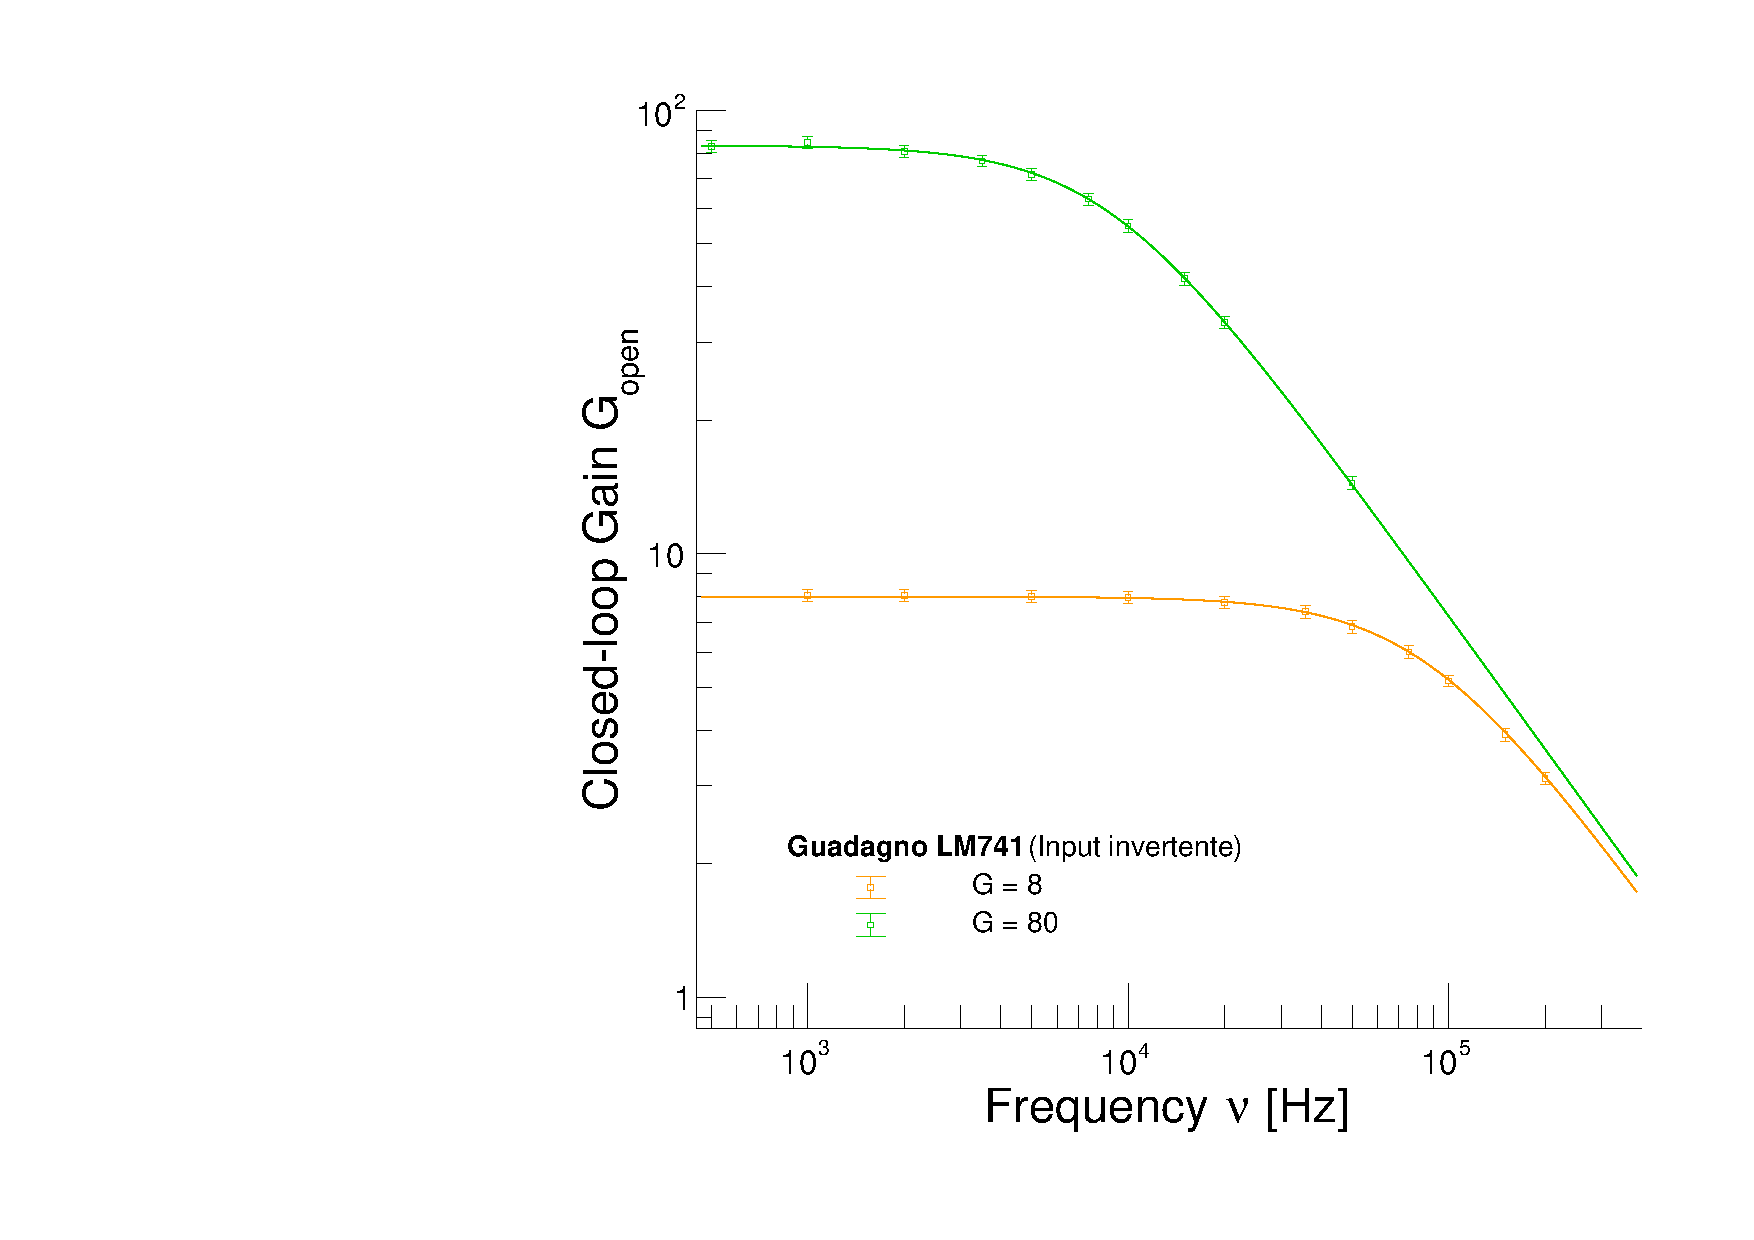
\includegraphics[width=\linewidth]{plot_combined.pdf}
    \caption{}
    \label{fig:plot_combined}
\end{figure}

Inoltre dalla \reffig{fig:plot_combined} possiamo osservare anche visualmente che il prodotto che prima abbiamo quantitativamente verificato essere costante sia visibile anche sovrapponendo i due diagrammi. Infatti possiamo osservare che diminuendo il guadagno $G_{\text{close}}$ da 80 a 8, ovvero cambiando $R_1$ da \SI{80}{\kilo\ohm} a \SI{8}{\kilo\ohm}, osserviamo che la frequenza di taglio si sposta di un fattore 10, passando da \SI{8}{\kilo\hertz} a \SI{80}{\kilo\hertz}.

Un'altra cosa che vogliamo misurare è il valore dell'impedenza di ingresso per verificare che come da modello sia effettivamente pari ad $R_1$. Per fare questo colleghiamo in serie una resistenza che abbia lo stesso valore di $R_1$ tra il punto che porta $V_{in}$ e $R_1$. Misuriamo quindi la tensione in uscita nel nodo di congiunzione tra le due resistenze e troviamo che il valore di $V_{out}$ è circa pari a $\frac{V_{in}}{2}$ e ciò significa che la tensione si è ripartita a metà tra la nuova resistenza che abbiamo inserito e l'impedenza di ingresso del circuito e quindi effettivamente l'impedenza di ingresso del nostro circuito è proprio $R_1$.

\begin{figure}[t!]
    \begin{circuitikz}
        \draw (0,0)
        node[op amp, scale=0.5, yscale=-1] (opamp) {}
        (opamp.-) -- (-1, -0.25) to [short, -*] (-1, -1)
        to [R, l^=$R_{1}$, resistors/scale=0.8] node[ground]{}(-1, -2.5)
        (-1, -0.25) -- (-1, -1) to [R, l=$R_{2}$, resistors/scale=0.8](1, -1)
        to [short, -*] (1, 0)
        (opamp.out) -- (2,0) node[right]{out}(2, 0)
        (opamp.+) -- (-1, 0.25) node[left]{in}
        ;
    \end{circuitikz}
    \caption{Schema circuitale amplificatore non-invertente}
    \label{fig:amp_noninv}
\end{figure}

Successivamente costruiamo un circuito amplificatore non-invertente il cui schema è riportato in \reffig{fig:amp_noninv} e utilizzando le stesse resistenze usate in precedenza. Ripetiamo quindi gli stessi procedimenti fatti prima per trovare il guadagno (dati raccolti in \reftab{??}) e troviamo che
\begin{align*}
    G &=\num{81.5167+-7.03287} \\
    q &=\SI{0.180687+-0.818311}{\volt} \\ 
\end{align*}

per cui il guadagno è compatibile con quello che avremmo dovuto ottenere da modello cioè $G=1+\frac{R_1}{R_2}$ mentre la quota è compatibile con zero.

Per misurare la tensione di ingresso del circuito ripetiamo ciò che avevamo fatto prima e questa volta troviamo che $V_{out}$ è praticamente uguale a  $V_{in}$. Ciò significa che la resistenza di ingresso del circuito è molto più grande di \SI{1}{\kilo\ohm} perchè infatti sulla nuova resistenza inserita non vi è praticamente caduta di potenziale. Ciò significa che il modello è verificato in quanto la resistenza di ingresso dovrebbe essere infinita, cioè realisticamente nell'ordine di $10^6 \Omega$.

Un'altra caratteristica dell'amplificatore che possiamo misurare è la cosiddetta "slew rate". La velocità di risposta, o slew rate, è una grandezza che indica la velocità, espressa in volt su secondi, con cui è capace di reagire un dispositivo o circuito elettronico, sollecitato sul suo ingresso, da un impulso di tensione, il cui valore, da minimo a massimo, è contenuto in un tempo brevissimo. Per misurarla costruiamo un comparatore a soglia nulla, il cui schema è riportato in \reffig{??} e mandiamo in ingresso un'onda quadra. Poichè quindi la risposta del circuito non è immediata, sull'oscilloscopio non osserviamo un'onda quadra, bensì dei trapezi isosceli e ciò che a noi interessa è proprio la pendenza dei lati obliqui di questi trapezi. Utilizzando i cursori dell'oscilloscopio possiamo quindi misurare il rapporto tra la variazione di tensione ($\Delta Y$) e l'intervallo di tempo ($\Delta X$). Troviamo quindi che il valore dello slew rate è \SI{0.54076305 +- 0.016294305}{\volt\micro\second^{-1}} che è molto vicino al valore indicato sul data-sheet del dispositivo.

\begin{figure}
    \begin{circuitikz}
        \draw (0,0)
        node[op amp, noinv input up, scale=0.75](opamp){\texttt{LM741}}
        (opamp.+) -- (-2, 0.375) node[left]{in}
        (opamp.-) -- (-2, -0.375) -- (-2, -0.75) node[ground]{}
        (opamp.out) -- (1, 0) node[right]{out}
        (opamp.up) -- ++(0, 1) node[above]{+Vcc}
        (opamp.down) -- ++(0, -1) node[below]{-Vcc}
        ;
    \end{circuitikz}
    \caption{Schema circuitale del comparatore utilizzato per effettuare la misura della \textit{slew rate}.}
    \label{fig:opamp_comparatore}
\end{figure}

\section*{Studio e caratterizzazione amplificatore per strumentazione}
Vogliamo costriure un amplificatore per strumentazione a due stadi il cui guadagno sia compreso tra 100 e 200. Infatti avere un guadagno troppo alto porta il segnale di uscita ad essere troppo sensibile a rumori e fluttazioni. Dallo studio del circuito riportato in \reffig{fig:opamp_comparatore} troviamo che se $R_{b}=R_{b}'$, $R_{c}=R_{c}'$ e $R_{d}=R_{d}'$ il guadagno è dato da \[G=\frac{R_{d}}{R_{c}}\cdot \left(1+2\cdot \frac{R_{b}}{R_{a}}\right).\] 

Prendiamo quindi come resistenze:
\begin{align*}
    R_a &= \SI{17.8 +- 0.109}{\kilo\ohm}\\
    R_b &= \SI{37.5 +- 0.166}{\kilo\ohm}\\
    R_c &= \SI{1.0 +- 0.064}{\kilo\ohm}\\
    R_d &= \SI{32.2 +- 0.151}{\kilo\ohm}\\
    R_b'&= \SI{37.5 +- 0.166}{\kilo\ohm}\\
    R_c'&= \SI{1.0 +- 0.064}{\kilo\ohm}\\
    R_d'&= \SI{32.2 +- 0.151}{\kilo\ohm}\\
\end{align*}
(Per assicurarci che le resitenze che volevamo fossero uguali avessero lo stesso valore abbiamo misurato ogni resistenza con il tester).

Il valore del guadagno dovrebbe quindi essere \num{1.68 +- 0.12e2}

Iniziamo misurando l'offset. L'offset è di fatto sempre presente perchè i due amplificatori che usiamo nel primo stadio, molto difficilmente sono identici e di conseguenza anche le correnti che scorrono in essi. Possiamo quindi usare un "trimmer" presente sulla scheda in modo da modificare la corrente in ingresso e cercare di eliminare l'offset. Per fare ciò





\begin{methods}{D\lowercase{ati completi e codice sorgente}}
    Tutti i dati completi a supporto dei grafici, e il relativo codice, sono visualizzabili su \url{https://github.com/mattiasotgia/Lab2}. L'analisi dati viene eseguita su un programma sviluppato in C++ basandosi su framework pubblici: ROOT, per la realizzazione dei grafici e il fit dei modelli (\url{https://root.cern/}).
\end{methods}

%\onecolumngrid
\appendix

% \setcounter{table}{0}
\renewcommand{\thetable}{S-\arabic{table}}

\end{document}
    
